\chapter{Overview}

\pulpissimo is a 32 bit \riscv single-core System-on-a-Chip.
\pulpissimo is the second version of the \pulpino system and it can be extended
with the multi-core cluster of the \pulp project.

Differently from the simpler \pulpino system, \pulpissimo uses
a more complex memory subsystem, an autonoumous I/O subsystem which uses the \udma, new peripherals (eg the camera interface) and a new SDK.

Figure~\ref{fig:pulpissimo_overview} shows a simplified block diagram of the SoC.
As for \pulpino, \pulpissimo can be configured at design time to use either the \riscy or
\zeroriscy.
The peripherals are connected to the \udma which transfers the date to the memory subsystem efficiently. The JTAG and the AXI plug have also access to the SoC.
The AXI plug can be used to extend the microcontroller with a multi-core cluster or an accelerator.
As for \pulpino, the advanced debug unit is used to access to system and core registers, memories and memory-mapped IO via JTAG.
A logarithmic interconnect allows to link the core and the \udma to the memory banks simultaneously.

\begin{figure}[H]
  \centering
  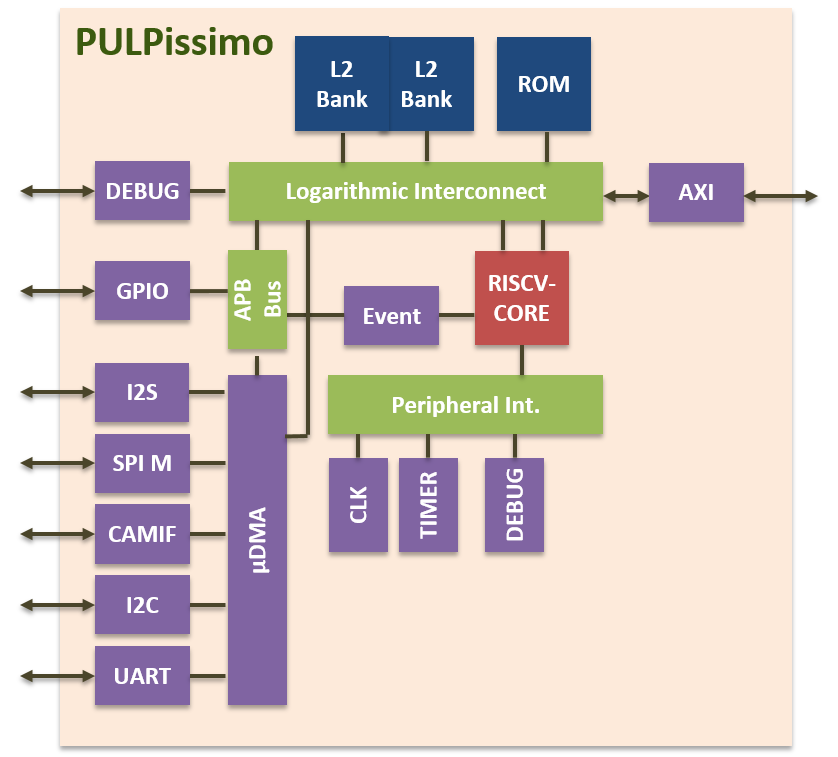
\includegraphics[width=0.9\textwidth]{./figures/pulpissimo_block.png}
  \caption{\pulpissimo Overview.}
  \label{fig:pulpissimo_overview}
\end{figure}


\pulpissimo is mainly targeted at RTL simulation and ASICs.
The FPGA versions has not yet been implemented.
